\newday{05 March 2024}
	\rule{0.5\textwidth}{0.5pt}\\

	{\large \textbf{EXPERIMENT PSFReconstructor-100-32-1}}\\
	
	{\normalsize HYPERPARAMETERS:}
	\begin{lstlisting}
	*ARCHITECTURE HYPERPARAMETERS:
		-Fully Connected
		-Input shape: 19
		-Output shape: 32768
		-Hidden layers: [128, 128, 128, 128, 256,
						256, 512, 2000, 4000]
		-Regularizer: None
		-Hidden Layers Activation: relu
		-Output Layer Activation: linear
		-Batch Normalization: False
		-Dropout: False, 0.2
	
	*COMPILATION HYPERPARAMETERS:
		-Optimizer: ADAM lr=0.001, beta_1=0.9, beta_2=0.999
		-Loss Function: MSE
		-Metric: MSE
	
	*TRAINING HYPERPARAMETERS:
		-Epochs: 10000
		-Batch size: 32
		-Callbacks: 
			-ReduceLROnPlateau: MSE 10 x0.1
			-Early Stop: MSE 25
	\end{lstlisting}
	
	{\normalsize VISUALIZATION:}
	\begin{lstlisting}
	*RESULTS:
        -Train MSE: 0.00033666446688584983
	\end{lstlisting}
	
	\begin{figure*}[ht!]
		\subfloat[Training Evolution]{%
		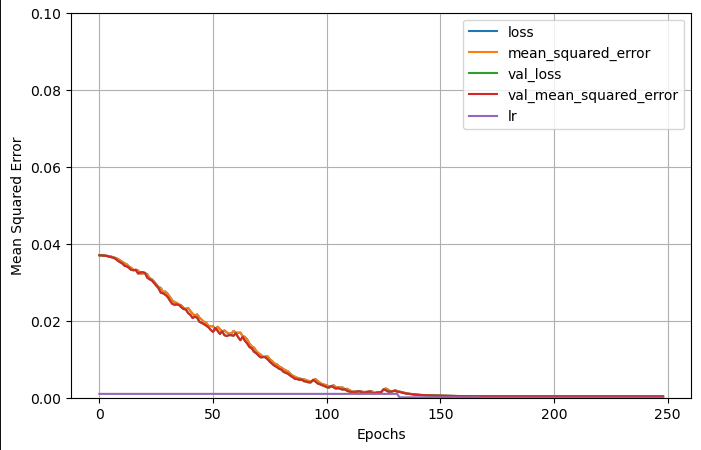
\includegraphics[ width=0.31\textwidth]{psf-PSFReconstructor-100-32-1-evolution.png}}
		\hspace{\fill}
		\subfloat[Train datapoint]{%
		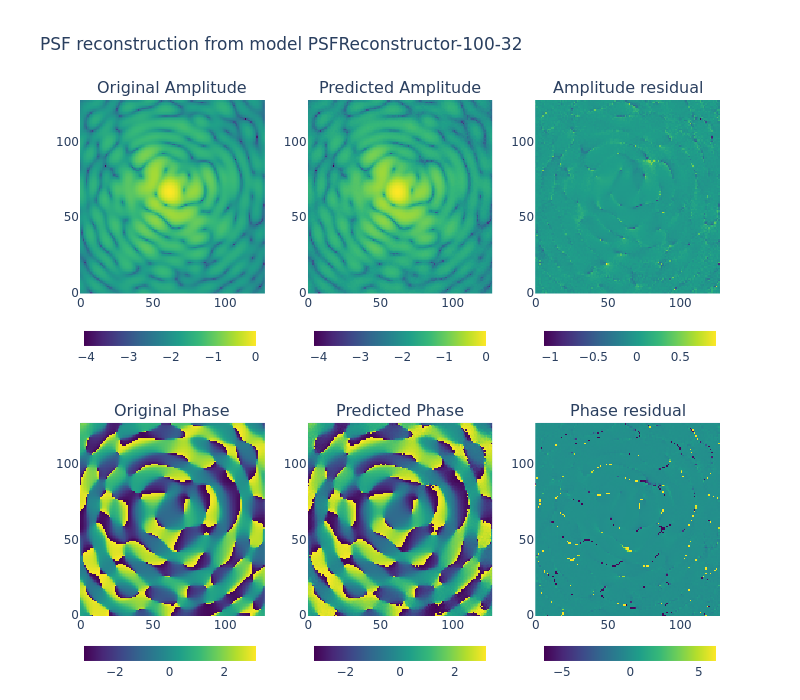
\includegraphics[ width=0.31\textwidth]{psf-PSFReconstructor-100-32-1-train.png}}
		\hspace{\fill}	
		\subfloat[Train datapoint]{%
		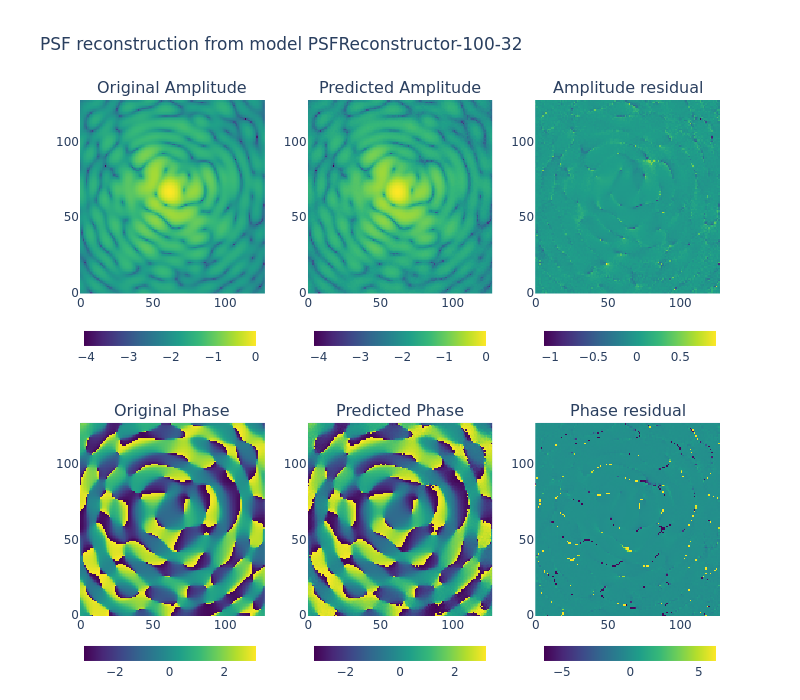
\includegraphics[ width=0.31\textwidth]{psf-PSFReconstructor-100-32-1-train.png}}\\
		\caption{Results of training the model PSFReconstructor-100-32-1}
	\end{figure*}
	
\FloatBarrier	
\rule{0.5\textwidth}{0.5pt}\\
	
	\rule{0.5\textwidth}{0.5pt}\\

	{\large \textbf{EXPERIMENT PSFReconstructor-100-16-1}}\\
	
	{\normalsize HYPERPARAMETERS:}
	\begin{lstlisting}
	*ARCHITECTURE HYPERPARAMETERS:
		-Fully Connected
		-Input shape: 19
		-Output shape: 32768
		-Hidden layers: [128, 128, 128, 128, 256,
						256, 512, 2000, 4000]
		-Regularizer: None
		-Hidden Layers Activation: relu
		-Output Layer Activation: linear
		-Batch Normalization: False
		-Dropout: False, 0.2
	
	*COMPILATION HYPERPARAMETERS:
		-Optimizer: ADAM lr=0.001, beta_1=0.9, beta_2=0.999
		-Loss Function: MSE
		-Metric: MSE
	
	*TRAINING HYPERPARAMETERS:
		-Epochs: 10000
		-Batch size: 16
		-Callbacks: 
			-ReduceLROnPlateau: MSE 10 x0.1
			-Early Stop: MSE 25
	\end{lstlisting}
	
	{\normalsize VISUALIZATION:}
	\begin{lstlisting}
	*RESULTS:
        -Train MSE: 0.0003098844608757645
	\end{lstlisting}
	
	\begin{figure*}[ht!]
		\subfloat[Training Evolution]{%
		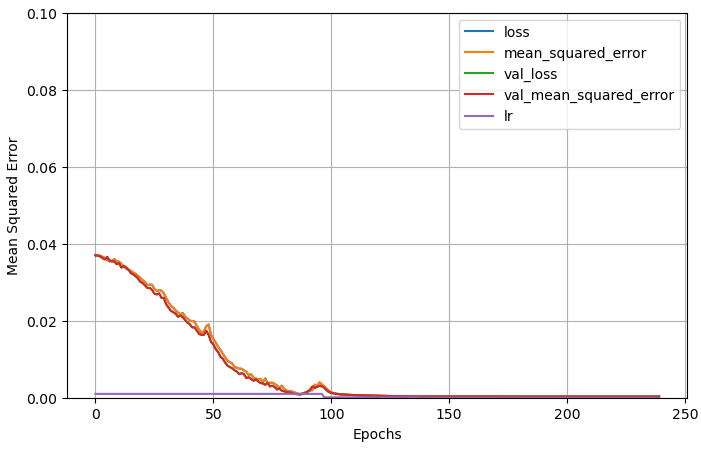
\includegraphics[ width=0.31\textwidth]{psf-PSFReconstructor-100-16-1-evolution.png}}
		\hspace{\fill}
		\subfloat[Train datapoint]{%
		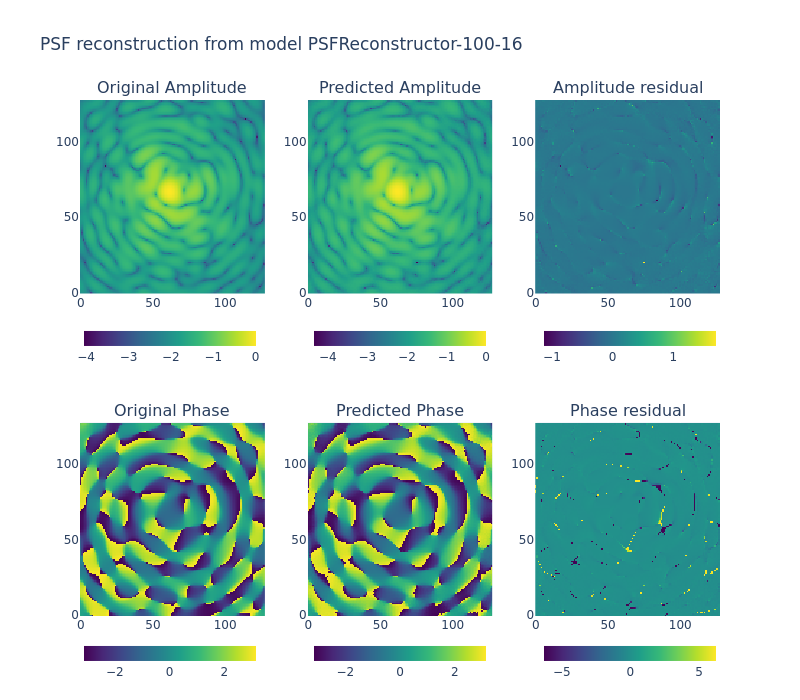
\includegraphics[ width=0.31\textwidth]{psf-PSFReconstructor-100-16-1-train.png}}
		\hspace{\fill}	
		\subfloat[Train datapoint]{%
		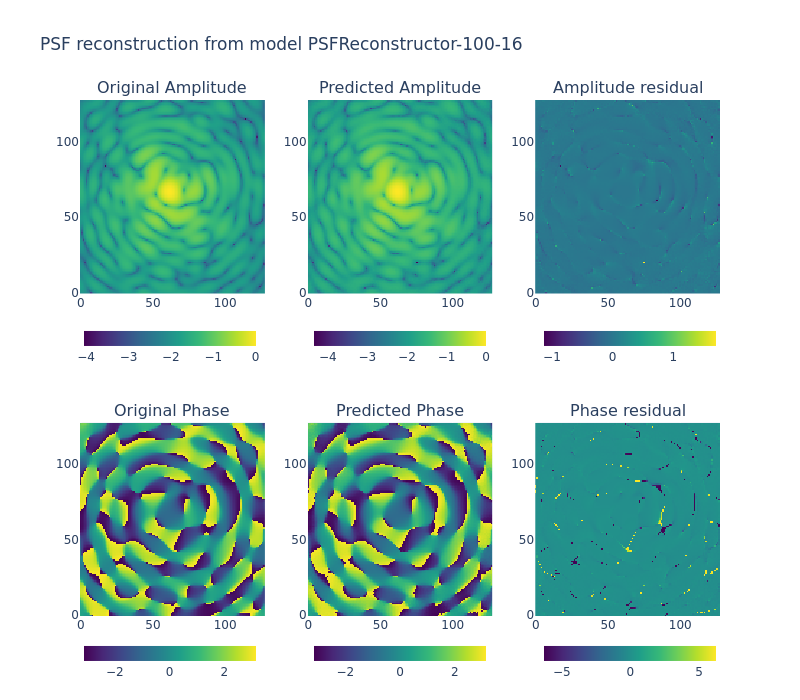
\includegraphics[ width=0.31\textwidth]{psf-PSFReconstructor-100-16-1-train.png}}\\
		\caption{Results of training the model PSFReconstructor-100-16-1}
	\end{figure*}
	
\FloatBarrier	
\rule{0.5\textwidth}{0.5pt}\\
	
	\action{
		Apart from the mse, no significant difference can be appreciated for different batch sizes using 100 datapoints.
	}
	
	\action{
		The goal for today is to study the correlation between the L2 norm of the pupil plane electric field and the L2 norm of the LP modes complex coefficients.
	}
		
	\action{
		First compute the L2 norm of the LP modes complex coefficients from the validation psf electric fields.
	}
	
	\action{
		Done!, here it is what it looks like
		\begin{figure}[!ht]
		\centering
			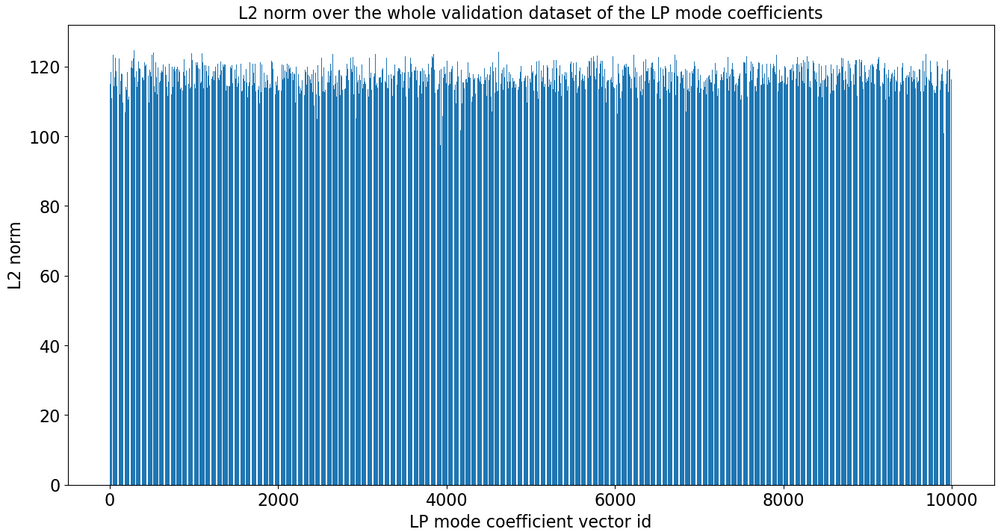
\includegraphics[scale=0.2]{L2-norms-mode-coefficients.png}
			\caption{L2 norms for the overlap integral mode coefficients of the validation PSFs}
			\end{figure}
	}
	
	\FloatBarrier
	\action{
		Let's do the same for the electric fields of the PSF
	}
	
	\action{
		Done!, here are the results:
		\begin{figure}[!ht]
		\centering
			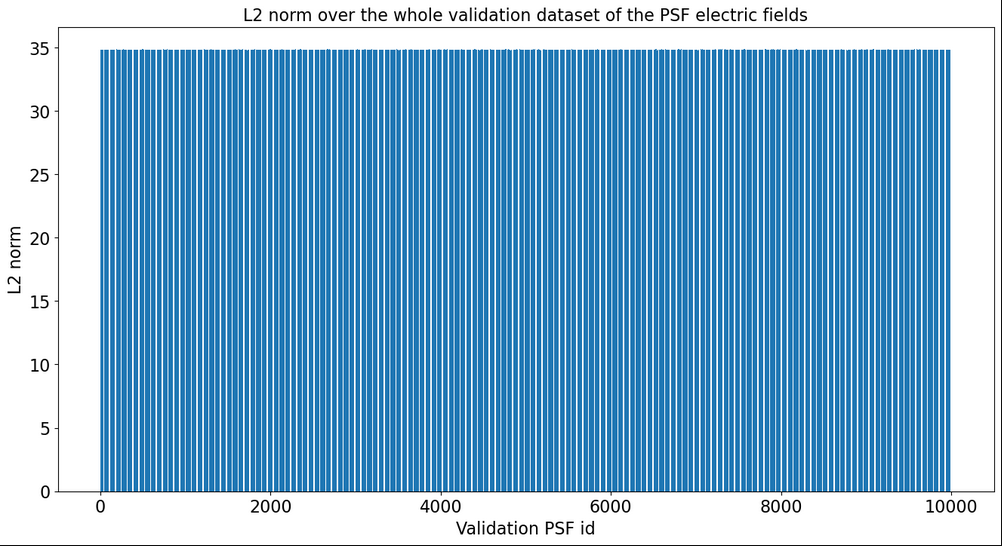
\includegraphics[scale=0.2]{L2-norms-PSFs.png}
			\caption{L2 norms of the validation PSFs electric fields}
			\end{figure}
	}
	\FloatBarrier
	
	\action{
		After doing a correlation analysis the result is the following:\\
		\filename{Pearson correlation coefficient: 0.1451513895198259}\\
		Which means that there is no correlation
	}
\finishday